\documentclass[a4paper,10pt,twoside]{article}
%%%%%%%%%%% Packages %%%%%%%%%%
\usepackage[margin=1in]{geometry}
\usepackage{amsmath, amssymb,mathtools}
\usepackage{fancyhdr}
\usepackage{sectsty}
\usepackage{enumitem}
\usepackage{float}
\usepackage{braket}
\usepackage{bbm}
\usepackage{tikz,calc}

%%%%%%%%%%% Macros %%%%%%%%%%
\def \note#1 {\vspace{-1em}\paragraph{\bfseries #1}}
\def \dd {{\rm d}}
\def \id {{\mathbbm{1}}}
\def \order {\mathcal{O}}
\def \A {\mathcal{A}}
\def\bquad{\mkern-18mu}
\DeclareMathOperator{\trace}{tr}
\DeclareMathOperator{\rank}{rank}

%%%%%%%%%%% Tikz Definitions %%%%%%%%%%
\usetikzlibrary{shapes, arrows,positioning,fit}
\tikzstyle{plain} = [draw,thick,circle,inner sep=0,minimum size=0.5cm,font=\footnotesize]
\tikzstyle{mps} = [draw,thick,circle,fill=blue!40,inner sep=0,minimum size=0.5cm]
\tikzstyle{mpo} = [draw,thick,diamond,fill=red!60,inner sep=0,minimum size=0.5cm]
\tikzstyle{blob} = [draw,thick,rectangle,rounded corners=.25cm,fill=blue!40]
\tikzstyle{index} = [-,thick,font=\footnotesize]
\tikzstyle{virtual} = [-,thick,dotted,font=\footnotesize]

\def\pair{\tikz[baseline=-0.5ex]{
\fill (0,0) circle (1.5pt) coordinate (A);
\fill (1.5ex,0) circle (1.5pt) coordinate (B);
\draw (A)--(B);}
}

%%%%%%%%%%% Formatting %%%%%%%%%%
\pagestyle{fancy}
\renewcommand{\footrulewidth}{0.5pt}

\fancyhf{}
\lhead{27/04/2017}
\chead{Quantum Information Methods in Many-Body Physics}
\rhead{PH2269}
\lfoot{Giacomo Giudice~~~~giacomo.giudice@mpq.mpg.de}
\rfoot{Page \thepage}

\allsectionsfont{\normalfont\sffamily}

%%%%%%%%%%% Here Begins Document %%%%%%%%%%
\begin{document}
\title{\vspace{-1cm}\sffamily Solutions to Homework 2\vspace{-1cm}}
\author{}
\date{}
\maketitle
\thispagestyle{fancy}


\begin{section}{}
The rank of the resulting tensor is simply the number of open legs in the diagram.
\begin{figure}[h]
  \centerline{
    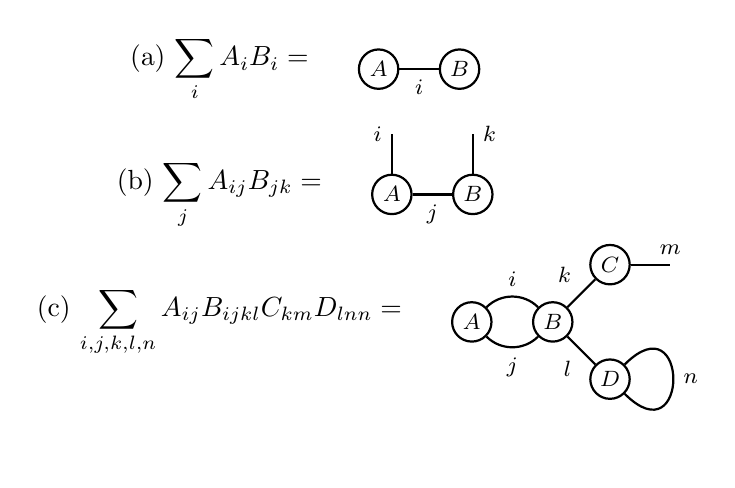
\begin{tikzpicture}[auto, node distance=0.5cm]
      \node (ex1) {(a)~$\displaystyle\sum_i A_i B_i = $};
      \node[plain,right=of ex1]  (v1) {$A$};
      \node[plain,right=of v1]  (v2) {$B$};
      \draw[index] (v1.east) -- (v2.west) node[midway,below]{$i$};
      \node[below= of ex1] (matmul) {(b)~$\displaystyle\sum_j A_{ij} B_{jk} = $};
      \node[plain,right=of matmul]  (m1) {$A$};
      \node[plain,right=of m1] (m2) {$B$};
      \draw[index] (m1.east) -- (m2.west) node[midway,below]{$j$};
      \draw[index] (m1.north) -- +(0,0.5) node[left]{$i$};
      \draw[index] (m2.north) -- +(0,0.5) node[right]{$k$};
      \node[below=of matmul] (ex2) {(c)~$\displaystyle\sum_{i,j,k,l,n} A_{ij} B_{ijkl} C_{km} D_{lnn}=$};
      \node[plain,right=of ex2]  (a) {$A$};
      \node[plain,right=of a]  (b) {$B$};
      \node[plain,above right=of b]  (c) {$C$};
      \node[plain,below right=of b]  (d) {$D$};
      \draw[index,out=45, in=135] (a) to node[above]{$i$} (b);
      \draw[index,out=-45, in=-135] (a) to node[below]{$j$} (b) ;
      \draw[index] (b.north east) -- (c.south west) node[midway,above left]{$k$};
      \draw[index] (b.south east) -- (d.north west)  node[midway,below left]{$l$};
      \draw[index] (c.east) -- +(0.5,0) node[above]{$m$};
      \draw[index,out=-45,in=45,loop] (d) to node[right]{$n$} (d);
    \end{tikzpicture}
  }
  \centerline{
    \begin{tikzpicture} [auto, node distance=0.5cm]
    \foreach \a [count=\c] in {A,B,C,D,E}{
      \node[plain] at (180-\c*360/5:1) (\a) {$\a$};
    }
    \def\lasta{E}
    \foreach \a [count=\c,remember=\a as \lasta] in {A,B,C,D,E}{
      \draw[index] (\a) -- (\lasta);
    }
    \node[fit=(A)(B)(C)(D)(E)] (f) {};
    \node[left=of f] (eq) {$\trace(ABCDE) = $};
  \end{tikzpicture}
}
\end{figure}

In practice we will seldom write explicitly the indices of a tensor networks.
This can lead to some confusion as to which contraction a diagram actually represents since it can be unclear which index is which.
For example we may be incorrectly lead to believe that figure above also represents the contraction $\trace(AEDCB)$. By writing down the indices explicitly, one can check that it is indeed a different contraction.
\end{section}

\begin{section}{}
\paragraph{Act I} 
Notice that the maximum number of Schmidt values (i.e. the Schmidt rank) is necessarily bounded by $\rank(c)$.
It follow that $E(\ket{\psi}) \leq \log_2 D_{\min}$, where $D_{\min} = \min(D_1,D_2)$.
By applying the mapping, we obtain $P\ket{\psi} = (P_1 c P_2^\top)_{n^\prime,m^\prime} \ket{n^\prime}\ket{m^\prime}$.
Using the property $\rank(AB) \leq \min\big(\rank(A),\rank(B)\big)$, the Schmidt rank is then bounded by 
\[
  \rank(P_1 c P_2^\top) \leq \min\big(\rank(c),\rank(P_1),\rank(P_2)\big) \leq D_{\min}
\]
Hence, $E(P\ket{\psi}) \leq \log_2 D_{\min}$.

\paragraph{Act II}
\begin{itemize}
  \item Using the previous point, $E(\pair) \leq \log_2 D$.
  \item Divide $\A$ into the boundary and the bulk: $\A = \partial \A + \A^\circ$.
  The bulk is in a pure state ($S_{\A^\circ} = 0$) and will not contribute to the entanglement: $S_A \leq S_{\partial \A} + S_{\A^\circ}$, hence $S_\A = S_{\partial\A} $. 
  A similar procedure applies to the pairs in $\bar{\A}$.
  \item We are cutting $|\partial A|$ entangled pairs, hence the entanglement will be bounded by $E_\A \leq |\partial \A| \log_2 D$.
\end{itemize} 

\paragraph{Act III} As we proved in Act I, local operations do not increase the entanglement.
We can split the total mapping into the terms acting inside $\A$ and the ones acting outside: $A_1 \otimes A_2 \otimes \dots \otimes A_N = M_\A \otimes M_{\bar{\A}}$.
By splitting the Hilbert space accordingly into $\ket{\varphi} = \sum c_{n,m} \ket{n}_\A \ket{m}_{\bar{\A}}$, we see that the mapping acts locally --- much as in Act I --- and the entropy cannot increase. 
Therefore, we obtain the area law for PEPS 
\[ 
  E_\A \leq |\partial \A| \log_2 D.
\]

\end{section}

\begin{section}{}
The mapping $M$ projects on the spin-1 subspace:
\[
  M^+=
  \begin{pmatrix}
    1 & 0\\
    0 & 0
  \end{pmatrix}, \quad
  M^0=\frac{1}{\sqrt{2}}
  \begin{pmatrix}
    0 & 1\\
    1 & 0
  \end{pmatrix}, \quad
  M^-=
  \begin{pmatrix}
    0 & 0\\
    0 & 1
  \end{pmatrix},
\]
\end{section}
The state $\ket{\Psi} = \mathcal{M} \ket{\Phi}$ is then 
\[
  \ket{\Psi} = \sum_{\boldsymbol{\sigma},\mathbf{a},\mathbf{b}} M^{\sigma_1}_{a_1,b_1} \Sigma_{b_1,a_2} M^{\sigma_2}_{a_2,b_2} \Sigma_{b_2,a_3} \dots \Sigma_{b_{L-1},a_L} A^{\sigma_L}_{a_L,b_L}  \Sigma_{b_L,a_1} \ket{\boldsymbol{\sigma}}
  = \sum_{\boldsymbol{\sigma}} \trace{\left(M^{\sigma_1} \Sigma M^{\sigma_2} \Sigma \dots M^{\sigma_L} \Sigma \right)} \ket{\boldsymbol{\sigma}}
\]
By introducing $A^\sigma = M^\sigma \Sigma$ we obtain the desired form.
\[
  A^+=\frac{1}{\sqrt{2}}
  \begin{pmatrix}
    0 & 1\\
    0 & 0
  \end{pmatrix}, \quad
  A^0=\frac{1}{2}
  \begin{pmatrix}
    -1 & 0\\
    0 & 1
  \end{pmatrix}, \quad
  A^-=\frac{1}{\sqrt{2}}
  \begin{pmatrix}
    0 & 0\\
    -1 & 0
  \end{pmatrix}.
\]
\begin{section}{}
\begin{enumerate}[label=(\alph*)]
\item A bond dimension $D=1$ is sufficient: $A^0 = 0$, $A^1 = 1$.
\item Here we need to introduce a mimimum of $D=2$
\[
  A^0=
  \begin{pmatrix}
    1 & 0\\
    0 & 0
  \end{pmatrix}, \quad
  A^1=
  \begin{pmatrix}
    0 & 0\\
    0 & 1
    \end{pmatrix}
\].
\item The most compact representation of the $\ket{\rm W}$ state is not translationally invariant. We then have to resort to different tensors and write $\ket{\rm W} = \sum \trace(A^{i_A}B^{i_B}C^{i_C}) \ket{i_A,i_B,i_C}$, with
\begin{align*}
  A^0&=
  \begin{pmatrix}
    1 & 0 & 0\\
    0 & 1 & 0\\
    0 & 0 & 0
  \end{pmatrix}, \quad
  B^0=
  \begin{pmatrix}
    1 & 0 & 0\\
    0 & 0 & 0\\
    0 & 0 & 1
    \end{pmatrix}, \quad
  C^0=
  \begin{pmatrix}
    0 & 0 & 0\\
    0 & 1 & 0\\
    0 & 0 & 1
    \end{pmatrix},\\
  A^1&=
  \begin{pmatrix}
    0 & 0 & 0\\
    0 & 0 & 0\\
    0 & 0 & 1
  \end{pmatrix}, \quad
  B^1=
  \begin{pmatrix}
    0 & 0 & 0\\
    0 & 1 & 0\\
    0 & 0 & 0
    \end{pmatrix}, \quad
  C^1=
  \begin{pmatrix}
    1 & 0 & 0\\
    0 & 0 & 0\\
    0 & 0 & 0
    \end{pmatrix}.
\end{align*}
\end{enumerate}
\note{Note} The choice of the tensors is not unique, you may well find a different combination that works.
\end{section}


\begin{section}{}
The proposed solution the \textsc{Matlab} script \texttt{multent.m} provided. 
The easiest way to approach the problem is to define the tensor $c_{ijkl}$, reshape it into the desired matrix, and then perform an SVD decomposition. 
Care should be taken when constructing the state, since most routines use column-major versus row-major reshaping.

\end{section}
\begin{section}{}
Applying the definition of $\hat{b}_k$,
\[
  \epsilon_k = -\frac{2t}{R} \cos\left(\frac{2\pi k}{R} \right) .
\]
In the thermodynamic limit $R\to\infty$, the gap goes to zero.
Hence this Hamiltonian is \emph{gapless}.
Doing the inverse Fourier transform, we obtain
\[ 
  \ket{\Psi_0} = \frac{1}{\sqrt{N!}}\left(\frac{1}{\sqrt{R}}\sum_{i=1}^R \hat{a}_i^\dag \right)^N\!\!\ket{0} .
\]
We split the sum and write
\begin{align*}
  \ket{\Psi_0} &= \frac{R^{-N/2}}{\sqrt{N!}} \left(\sqrt{L} \hat{a}_A^\dag + \sqrt{R-L}\hat{a}_{\bar{A}}^\dag \right)^N\!\!\ket{0} \\
  &= \frac{R^{-N/2}}{\sqrt{N!}} \sum_{n=0}^N {N \choose n} \left(\sqrt{L} \hat{a}_A^\dag\right)^n \left(\sqrt{R-L} \hat{a}_{\bar{A}}^\dag\right)^{N-n}\bquad \ket{0} \\
  &=  \sum_{n=0}^N \frac{\sqrt{N!}}{\sqrt{n!} \sqrt{(N-n)!}} \left(\frac{L}{R}\right)^{\frac{n}{2}} \left(\frac{R-L}{R}\right)^{\frac{N-n}{2}} \frac{(\hat{a}_A^\dag)^n}{\sqrt{n!}} \frac{(\hat{a}_{\bar{A}}^\dag)^{N-n}}{\sqrt{(N-n)!}}\ket{0} \\
  &=  \sum_{n=0}^N \sqrt{\lambda_n} \ket{n}_A\ket{N-n}_{\bar{A}},
  \quad \lambda_n = {N\choose n} \left(\frac{L}{R}\right)^{n} \left(1-\frac{L}{R}\right)^{N-n}
\end{align*}
This is explicitly a Schmidt decomposition, i.e. $\rho_n = \lambda_n$.
Notice also that $\lambda_n$ follows a binomial distribution with parameter $p=L/R$, therefore as $N \to \infty$ it approaches a normal distribution $\mathcal{N}\big(N p, Np(1-p) \big)$.
Computing the entropy is a Gaussian integral. Using $\int_{-\infty}^\infty e^{-x^2/\alpha^2} = \sqrt{\pi/\alpha}$ and $\int_{-\infty}^\infty x^2 e^{-x^2/\alpha^2} = \sqrt{\pi}/\alpha^{3/2}$,
\[
  E_A = \int_{-\infty}^\infty \frac{1}{\sqrt{2 \pi \sigma^2}} e^{ -\frac{n^2}{2\sigma^2}} \left(\frac{1}{2\sigma^2}n^2 +\log\sqrt{2\pi\sigma^2}\right) \dd n = \frac{1}{2} + \log\sqrt{2\pi\sigma^2} = \log\sigma + \frac{1+\log(2\pi)}{2} .
\]

Since $\sigma^2 = \frac{N}{R}(1-\frac{L}{R})L \to  \frac{N}{R}L$ when $N,R \to \infty$
\[
  E_A = \frac{1}{2}\log(L) + \frac{\log(N/R) + \log(2\pi)+ 1}{2}.
\]
In this case, \emph{the area law is violated}. 
From the calculations shown above, the Hamiltonian is gapless, so we can't apply the known theorems to show an area law. 

\note{Note} If you used the base-2 logarithm, you have to rescale this result by a factor $\log_2 e$.
\end{section}
\end{document}
%%%%%%%%%%% Here Ends Document %%%%%%%%%%
